\documentclass[a4paper,twocolumn]{article}

\usepackage{color}
\usepackage{appendix}

\usepackage{amsmath}

\usepackage{listings}
\usepackage{graphicx}
\usepackage[sc]{mathpazo} % Use the Palatino font
\usepackage[T1]{fontenc} % Use 8-bit encoding that has 256 glyphs
\usepackage[utf8]{inputenc} % Use utf-8 as encoding
\linespread{1.05} % Line spacing - Palatino needs more space between lines
\usepackage{microtype} % Slightly tweak font spacing for aesthetics

\usepackage[spanish]{babel} % Language hyphenation and typographical rules
%\usepackage[galician]{babel} % Change to this if using galician

\usepackage[hmarginratio=1:1,top=32mm,columnsep=20pt]{geometry} % Document margins
\usepackage[hang, small,labelfont=bf,up,textfont=it,up]{caption} % Custom captions under/above floats in tables or figures
\usepackage{booktabs} % Horizontal rules in tables

\usepackage{enumitem} % Customized lists
\setlist[itemize]{noitemsep} % Make itemize lists more compact

\usepackage{parskip}

\usepackage{abstract} % Allows abstract customization
\renewcommand{\abstractnamefont}{\normalfont\bfseries} % Set the "Abstract" text to bold
\renewcommand{\abstracttextfont}{\normalfont\small\itshape} % Set the abstract itself to small italic text

\usepackage{titlesec} % Allows customization of titles
\renewcommand\thesection{\Roman{section}} % Roman numerals for the sections
\renewcommand\thesubsection{\Alph{subsection}} % roman numerals for subsections
\titleformat{\section}[block]{\large\scshape\centering}{\thesection.}{1em}{} % Change the look of the section titles
\titleformat{\subsection}[block]{\large}{\thesubsection.}{1em}{} % Change the look of the section titles

\usepackage{fancyhdr} % Headers and footers
\pagestyle{fancy} % All pages have headers and footers
\fancyhead{} % Blank out the default header
\fancyfoot{} % Blank out the default footer
%\fancyhead[C]{Running title $\bullet$ May 2016 $\bullet$ Vol. XXI, No. 1} % Custom header text
\fancyfoot[C]{\thepage} % Custom footer text

\usepackage{titling} % Customizing the title section

\usepackage{hyperref} % For hyperlinks in the PDF

\usepackage[verbose]{placeins}

%----------------------------------------------------------------------------------------
%	TITLE SECTION
%----------------------------------------------------------------------------------------

\setlength{\droptitle}{-5\baselineskip} % Move the title up

%\pretitle{\begin{center}\huge\bfseries} % Article title formatting
%\posttitle{ \end{center} } % Article title closing formatting

\title{
    \begin{center}
        \huge\bfseries Procesadores del lenguaje: Prácticas 1 y 2
    \end{center}
} % Article title

\preauthor{\setlength{\parskip}{20pt}}

\postauthor{\setlength{\parskip}{1pt}}


\author{%
    \begin{center}
        \large\centering\textsc{Marcelo Fort Muñoz} \\[1ex] % Your name
        \normalsize Procesadores del lenguaje \\[0.25ex]
        \normalsize Universidad de Nebrija (Grupo A2) \\[0.25ex] % Your institution
        \normalsize \{mfortm\}@alumnos.nebrija.es % Your email address
        %\and % Uncomment if 2 authors are required, duplicate these 4 lines if more
        %\textsc{Jane Smith}\thanks{Corresponding author} \\[1ex] % Second author's name
        %\normalsize University of Utah \\ % Second author's institution
        %\normalsize \href{mailto:jane@smith.com}{jane@smith.com} % Second author's email address
    \end{center}
}

\predate{\setlength{\parskip}{5pt}}
\postdate{\setlength{\parskip}{1pt}}

\date{\begin{center}
          \large\today\\[2.5ex]
\end{center}} % Leave empty to omit a date

\renewcommand{\maketitlehookd}{%
    \begin{abstract}
        \setlength{\parskip}{22pt}
        \noindent Los \textbf{analizadores léxicos}, o «\textbf{lexers}», constituyen la primera fase en el proceso de compilación.
        Su función principal es procesar el código fuente, limpiarlo y descomponerlo en tokens, que luego son pasados al \textbf{analizador sintáctico} o «\textbf{parser}». Posteriormente, el analizador sintáctico utiliza estos tokens para construir \textbf{árboles de sintaxis} mediante acciones semánticas.
        En el caso de analizadores «Top-Down», es fundamental eliminar la recursividad por la izquierda para evitar bucles infinitos y asegurar una correcta traducción. \\\mbox{}\\
        \textbf{\textit{Palabras clave}: Compiladores, Análisis léxico, Análisis sintáctico, Árboles de sintaxis, Traducción dirigida por la sintaxis}
        \setlength{\parskip}{10pt}
    \end{abstract}

}

%----------------------------------------------------------------------------------------

\definecolor{dkgreen}{rgb}{0,0.6,0}
\definecolor{gray}{rgb}{0.5,0.5,0.5}
\definecolor{mauve}{rgb}{0.58,0,0.82}

\lstset{frame=tb,
    language=C,
    aboveskip=3mm,
    belowskip=3mm,
    showstringspaces=false,
    columns=flexible,
    basicstyle={\small\ttfamily},
    numbers=none,
    numberstyle=\tiny\color{gray},
    keywordstyle=\color{blue},
    commentstyle=\color{dkgreen},
    stringstyle=\color{mauve},
    breaklines=true,
    breakatwhitespace=true,
    tabsize=3
}



\begin{document}

    % Print the title
    \maketitle

    \parskip=0.5\baselineskip \advance\parskip by 0pt plus 1pt
%\setlength{\parskip}{1pt}
%----------------------------------------------------------------------------------------
    %	ARTICLE CONTENTS
    %----------------------------------------------------------------------------------------


    \section{Introducción}\label{sec:introduccion}

    En este trabajo se intentará sintetizar con la mayor claridad posible una descripción sobre el proceso de análisis léxico apoyándose en una versión del lexer proporcionado para ello\cite{codigos}.
    Después, se explicará cómo se ha modificado una implementación de un esquema de traducción dirigida por sintaxis, parte de los analizadores sintácticos (parseres), provisto para este informe para eliminar la recursividad a la izquierda.
    También se han añadido acciones semánticas para realizar su labor de traducción de notación infija a postfija (o polaca inversa).

    El lexer descompondrá el texto en componentes indivisibles (tokens).
    Este texto es almacenado en una cadena y cada uno de sus caracteres es procesado secuencialmente para identificar \textbf{palabras reservadas, identificadores, operadores, delimitadores, y números}.
    Este también tendrá que limpiar tabulaciones, retornos de carro y saltos de línea, contabilizando las líneas para mayor información.

    Por otro lado, el esquema de traducción dirigida por la sintaxis, obtiene los tokens provistos por el lexer y, mediante ellos, procede a construir un árbol con las expresiones; estos siguen una gramática específica.


    En los parsers Top-Down (como el usado en la práctica y en los que se enfoca este informe), se analiza en preorden (de \textbf{raíz} a \textbf{nodos}) y se suele usar el acercamiento LL, que significa:
    \begin{itemize}
        \item{Left-To-Right} El procesamiento de las cadenas se realiza de izquierda a derecha.
        \item{Leftmost derivation}
        Se aplica la regla producción que esté más a la izquierda.
    \end{itemize}En este caso, si hay una producción en la que hay el mismo símbolo no terminal a la derecha y como primer elemento a la izquierda, puede haber una recursión infinita (llamada recursividad a la izquierda), que no es deseable.


    En las producciones de la gramática se introducen acciones semánticas («operaciones adicionales» que se añaden a las producciones semánticas), que permiten la conversión de los tokens pasados por el lexer a un árbol de sintaxis abstracta \textit{AST\footnote{Del inglés: «Abstract Syntax Tree»}}, además de permitir realizar operaciones como la impresión de mensajes de error.


    \section{Metodología y funcionamiento}\label{sec:metodologia-y-funcionamiento}

    \subsection{Clasificación de los lexemas}\label{subsec:clasificacion-de-los-lexemas}
    Según el analizador léxico recorre el código fuente, este se puede ir topando con distintas secuencias de caracteres.
    Estos podrán ser clasificados en:
    \begin{enumerate}
        \item{Identificadores:} Formados por una o más letras seguídos de cero o más números, pueden incluir guiones bajos (\_) y que no pueden comenzar con números (0-9).
        Estos son sensibles a mayúsculas/minúsculas (a-z, A-Z) y no pueden ser palabras reservadas (esto puede variar para otros lexers).

        \item{Palabras reservadas:} Conjuntos de caracteres que tienen un significado especial para el lenguaje interpretado.
        En nuestro caso, las palabras reservadas disponibles se encuentran almacenadas en un diccionario.

        \item{Números:}
        Compuestos por dígitos, estos serán clasificados en flotantes o en enteros dependiendo de si contienen punto flotante (.).

        \item{Espacios, tabuladores y saltos de línea:}
        Estos son descartados, pero los saltos de línea son contabilizados.

        \item{Operadores y delimitadores:}
        Se reconocen operadores aritméticos, lógicos, relacionales, y delimitadores.

    \end{enumerate}

    \subsection{Procesamiento de un carácter}\label{subsec:procesamiento-de-un-caracter}
    Una vez el analizador «se hace» con un carácter, este procederá a analizarlo.


    De ser ``\#'', se devolverá ``<end\_program>'' (\autoref{subsec:pdtk} sobre la creación de los tokens), significando que se ha terminado de leer el archivo.
    Este comportamiento adoptado no es una convención generalizada, sino una decisión de diseño para facilitar la detección del final de archivo (\textit{end-of-file}).
    Por ejemplo, \textit{IBM} detecta el final del archivo con \%EOF\cite{IBM_EOF}, cada lexer puede detectar el fin de archivo de distinta forma.\par
    Lo más probable es que el carácter leído no sea ese carácter de final de archivo, sino que en su lugar sea una letra, número o carácter especial.
    En ese caso, de ser una letra, se irá iterando sobre la cadena seleccionada hasta toparse con un espacio o carácter no permitido, teniendo en este caso, que lanzarse un error léxico (es decir, el carácter no se ajusta a ninguno de los patrones que reconoce nuestro lexer).

    Una vez obtenida la cadena completa, de estar entre la lista de palabras reservadas, esta misma será su propia identificadora.
    En cualquier otro caso válido, se le asignará un ID.
    Se puede ver como se han clasificado las palabras reservadas en la \autoref{fig:palabrasReservadas}.

    \begin{figure}[h]
        \centering
        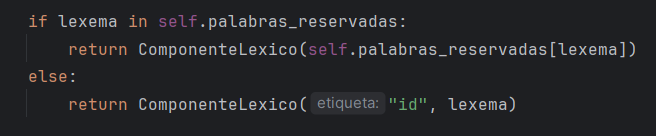
\includegraphics[width=1.00\linewidth]{esReservada}
        \caption{Palabras reservadas}
        \label{fig:palabrasReservadas}
    \end{figure}

    De ser un numérico, se interpretará como número.
    Se irán recogiendo los dígitos y, si se detecta la puntuación asignada al punto flotante, al terminar de procesarlos, se creará un componente léxico con etiqueta float en vez de int.
    En el valor se procederá a guardar el valor del número completo.

    A mayores, los caracteres también pueden ser operadores o delimitadores.
    Estos se procesan mediante una «\textit{serie}» de \textit{if-elses} que determinan el tipo del componente.

    En algunos casos como, por ejemplo, es el del mayor o igual, al estar compuesto de dos caracteres se ha de procesar primero el mayor, y después, ojear (\textit{lookahead}) el siguiente valor para ver si es el carácter igual (``='').
    De ser así, el token es mayor o igual ($>=$) (\autoref{fig:menorOigual}), y en caso negativo, solo mayor.

    En esta situación, todos los operadores tienen valor y etiqueta, mientras que los delimitadores carecen de valor.

    \begin{figure} [ht]
        \centering
        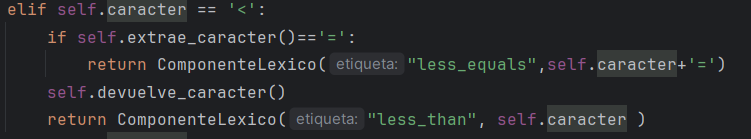
\includegraphics[width=1\linewidth]{imagen}
        \caption{Caso de menor o igual}
        \label{fig:menorOigual}
    \end{figure}



    A continuación, se muestra un diagrama de flujo
    para la decisión de creación de token:

    \clearpage
    \begin{figure}
        \centering
        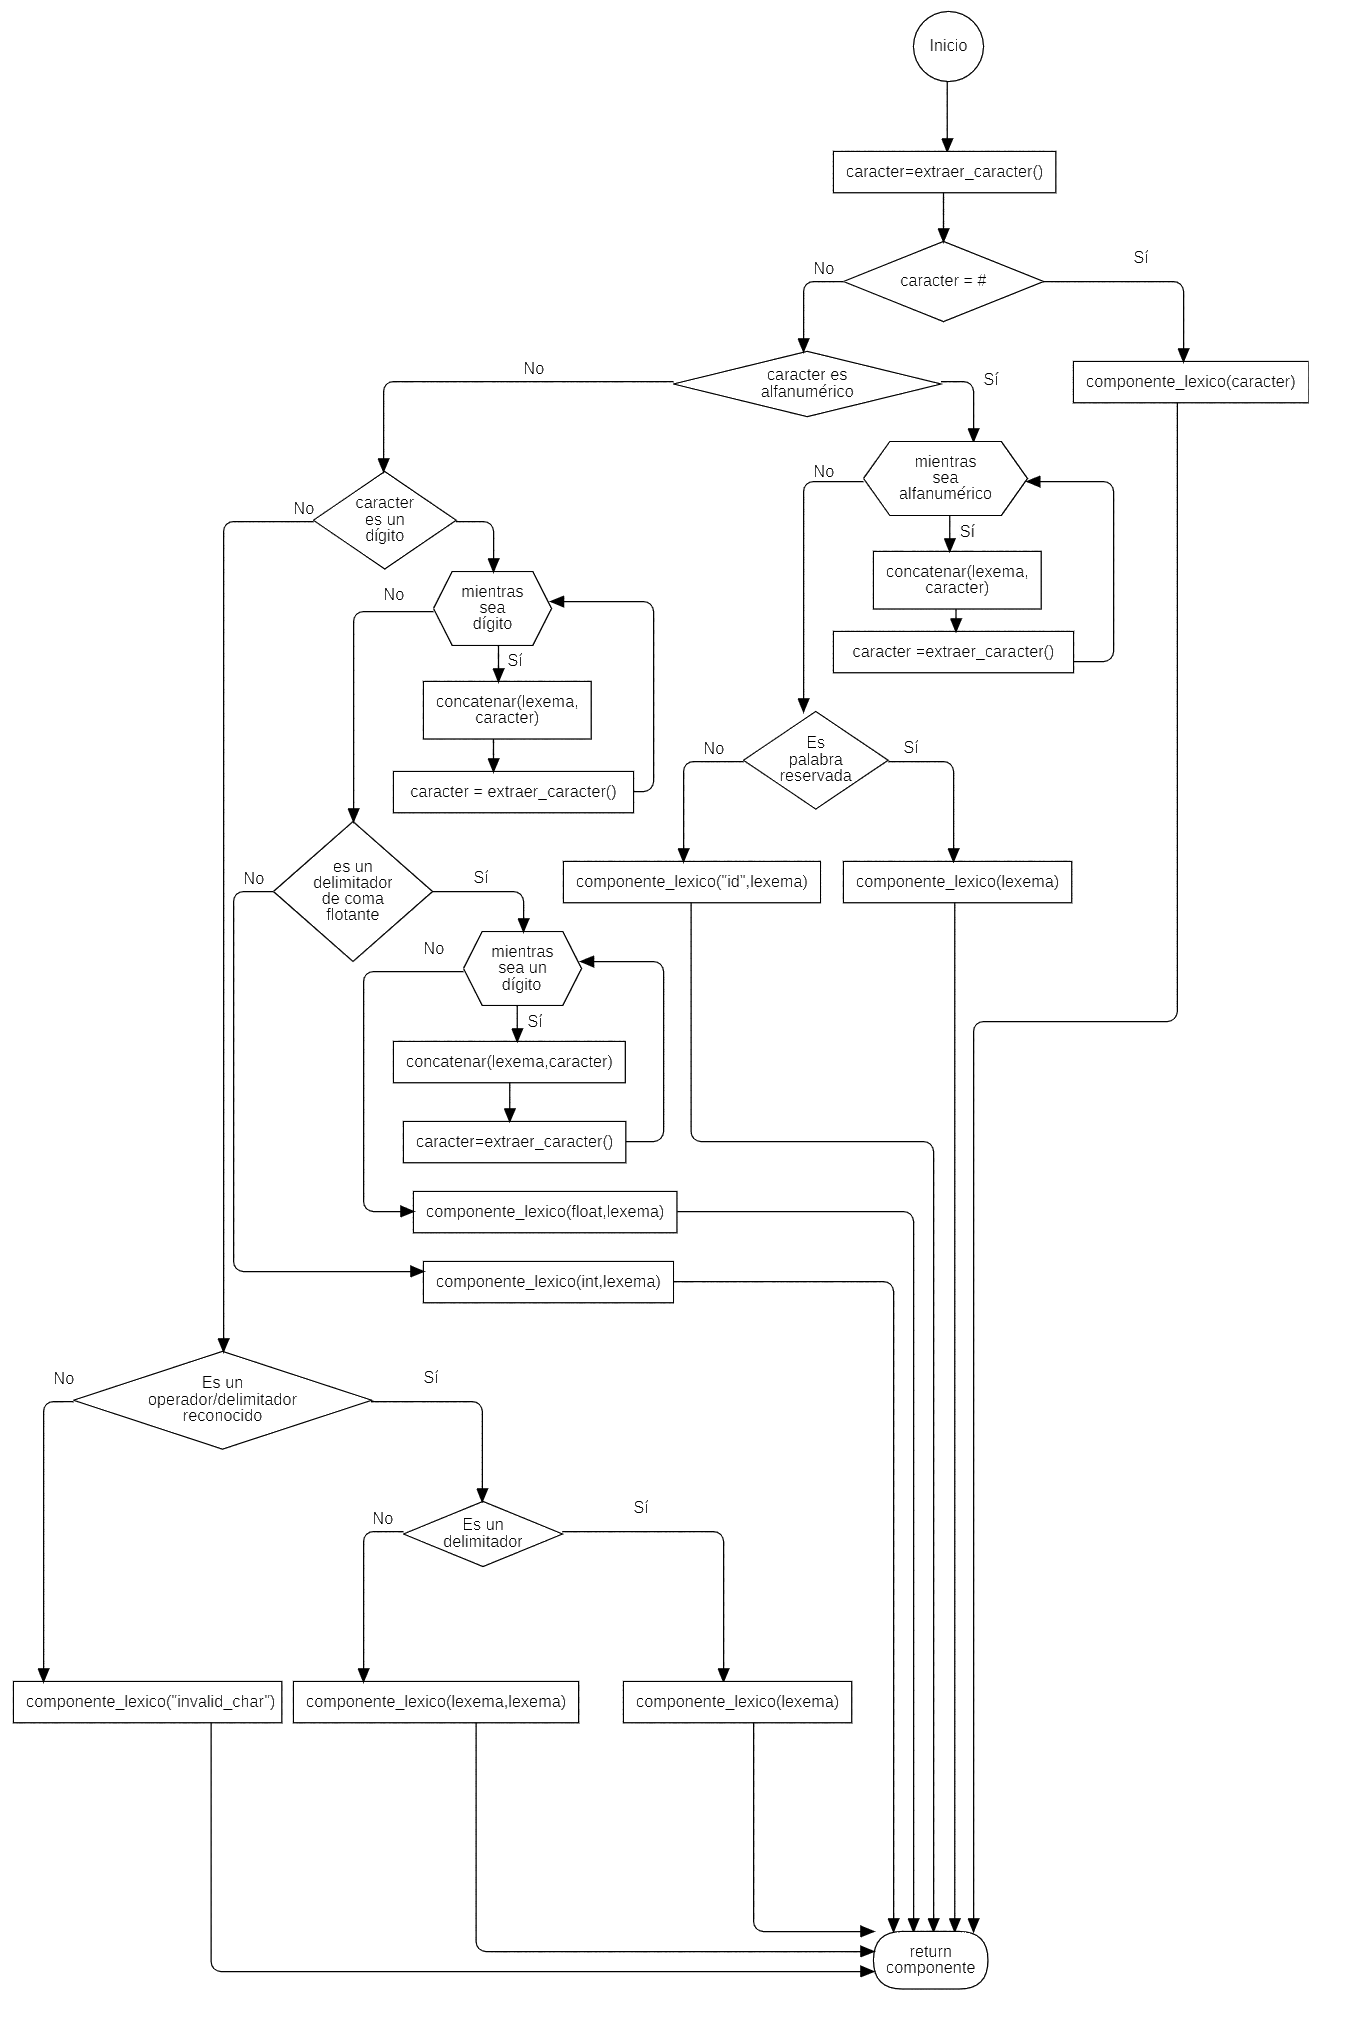
\includegraphics[width=1.00\linewidth]{diagramaFlujoDecisionCaracteresFinal}
        \caption{Diagrama de flujo para la creación de un token}
        \label{fig:diag 1}
    \end{figure}

    \subsection{Procesado de tokens}\label{subsec:pdtk}
    Cuando el analizador sabe qué es la cadena que tiene entre manos, este la usa para crear un token.
    Este consiste en un lexema (opcional) y su correspondiente etiqueta.

    Generalmente, el token está compuesto por: Como en nuestro caso de lexema y etiqueta, y además, de atributos como del número de línea, columna, etc.


    \section{Ejemplo de ejecución del traductor de notación}\label{sec:ejemplo-de-ejecucion-del-traductor-de-notacion}
    Se ha probado el analizador léxico implementado con el código que aparece en la Figura \autoref{fig:codC}.

    \begin{figure}
        \lstset{language=C}
        \begin{lstlisting}[label={lst:lstlisting}]
int i = h(x);
while ( A[i] != x ){
    if ( A[i] != 0 ){
        i = i - 1;
    }
    else if ( i = 0 ){
        i = m;
    }
    else{
        A[i] = x;
        B[i] = 0;
        break;
    }
}
B[i] = B[i]+1;
        \end{lstlisting}
        \caption{Código C usado por el Dr. Donald E. Knuth en su artículo\cite{donald}}
        \label{fig:codC}
    \end{figure}

    Dado el resultado de la ejecución del lexer usando el código de Donald (ver \autoref{app:a}), se puede observar que el resultado es el esperado y que no hay nada fuera de lo normal.
    El resultado obtenido se corresponde directamente con el código escrito por el Dr. Knuth.


    \section{Modificaciones realizadas a la gramática original}\label{sec:modificaciones-realizadas-a-la-gramatica-original}

    \subsection {Eliminando la recursión a la izquierda}\label{subsec:eliminando-la-recursion-a-la-izquierda}
    En esta sección se detallará como se modificó la gramática para eliminar la recursividad a la izquierda.

    Dicha gramática se puede ver en la \autoref{fig:gramatica_original}.

    \begin{figure}[hbtp]
        \begin{gather}
            \text{expresión} \quad \rightarrow \quad \text{expresión} + \text{término} \, \vert  \\
            \qquad \qquad \qquad \quad \; \; \; \text{expresión} - \text{término} \, \vert \\
            \quad \; \; \, \, \text{término} \\
            \nonumber\\
            \text{término} \quad \rightarrow \quad \text{término} * \text{factor} \, \vert \\
            \qquad \qquad \qquad \quad   \text{término} / \text{factor} \: \,\, \vert \\
            \quad \quad  \; \text{factor} \\
            \nonumber\\
            \text{factor} \quad \rightarrow \quad \text{( expresión )} \, \vert \\
            \qquad \quad \;  \; \text{num}
        \end{gather}
        \caption{Gramática original}
        \label{fig:gramatica_original}
    \end{figure}


    Como se puede ver en la \autoref{fig:gramatica_original}, existe recursividad a la izquierda en las producciones de expresión:
    \begin{align}
        &\text{expresión} \rightarrow \text{expresión} + \text{término} \\
        &\text{expresión} \rightarrow \text{expresión} - \text{término}
    \end{align}

    También existe esa recursividad hacia la izquierda en las producciones de término:

    \begin{align}
        &\text{término} \rightarrow \text{término} * \text{factor} \\
        &\text{término} \rightarrow \text{término} / \text{factor}
    \end{align}

    Para eliminar dicha recursividad, se utilizará la fórmula\cite{librodragon}:
    \begin{gather*}
        A \rightarrow \beta R\\
        R \rightarrow \alpha R \; \vert \; \epsilon
    \end{gather*}

    \subsubsection{Caso de expresión}
    En el caso de expresión, siguiendo las producciones originales de la \autoref{fig:gramatica_original}, podemos concluir que nuestros $ \alpha_i $ serán:
    \begin{align*}
        &\alpha_1 = + \: \text{término}\\
        &\alpha_2 = - \: \text{término}
    \end{align*}
    y $ \beta $ será:
    \[\beta = \text{término}\]

    Usando la fórmula antes señalada, nos quedarán las producciones no recursivas de la \autoref{fig:expr_nr_b}.

    \begin{figure}[h]
        \begin{align}
            &\text{expresión} \rightarrow \text{término} \; \text{expresión}' \\
            &\text{expresión}' \rightarrow + \; \text{término} \; \text{expresión}' \\
            &\vert \; - \; \text{término} \; \text{expresión}' \\
            &\vert \; \epsilon
        \end{align}

        \caption{Producciones de expresión sin recurrencia a la izquierda}
        \label{fig:expr_nr_b}
    \end{figure}

    \subsubsection{Caso de término}
    De la misma forma que para las producciones de expresión, primero extraemos los $\alpha$:
    \begin{align}
        \alpha_1 = * \; \text{factor}\nonumber \\
        \alpha_2 = / \; \text{factor}\nonumber
    \end{align}
    Para el caso de $\beta$:
    \begin{align}
        \beta = \text{factor} \nonumber
    \end{align}

    Usando esas $\alpha$ y $\beta$, se procesa la producción original en:

    \begin{figure}[ht]

        \begin{align}
            &\text{término} \rightarrow \text{factor} \; \text{término}' \\
            &\vert \; \text{término}' \rightarrow * \; \text{factor} \; \text{término}' \\
            &\vert \; / \; \text{factor} \; \text{término}'\\
            &\vert \; \epsilon
        \end{align}
        \caption{Producciones de término sin recurrencia a la izquierda}
        \label{fig:Term_nr_b}
    \end{figure}

    Como factor no tiene recursividad, lo dejamos como está.

    \subsubsection{Renombrado de producciones}
    Como ahora tenemos dos nuevas producciones llamadas \textit{expresión'} y \textit{término'}, para mayor facilidad de tratamiento, les cambiaremos el nombre.

    En el caso de \textit{expresión'}, como va después de \textit{término}, lo llamaremos \textit{más\_términos}.
    Para el caso de \textit{término'}, lo renombraremos como \textit{más\_factores}.

    \subsubsection{Resultado tras la eliminación de la recursividad}
    Tras eliminar la recursividad, obtenemos la gramática de la \autoref{fig:Term_nr_totales}

    \clearpage

    \begin{figure}
        \begin{align}
            \label{eqc:gramaticaCorregida}
            &\text{expresión} \rightarrow \text{término} \; \text{más\_términos} \\
            &\text{más\_términos} \rightarrow  + \;\text{término} \; \text{más\_términos}
            \refstepcounter{equation}\nonumber  \\
            &\vert \; - \text{término} \; \text{más\_términos} \\
            &\vert \; \epsilon \\
            &\text{término} \rightarrow \text{factor} \; \text{más\_factores} \\
            &\text{más\_factores} \rightarrow  * \;\text{factor} \; \text{más\_factores} \\
            &\vert \; / \; \text{factor} \; \text{más\_factores} \\
            &\vert \; \epsilon \\
            &\text{factor} \; \rightarrow (\text{expresión})\\
            &\vert \; num\label{eq:numSinRecursividad}
        \end{align}
        \caption{Gramática sin recursividad a la izquierda}
        \label{fig:Term_nr_totales}
    \end{figure}


    \section{Acciones añadidas a la gramática}\label{sec:acciones-anadidas-a-la-gramatica}
    Una vez modificada la gramática para que no haya producciones con recurrencia a la izquierda (\autoref{fig:Term_nr_totales}), procedemos a añadir acciones semánticas que nos permitan hacer la traducción guiada por la sintaxis.


    En primer lugar, se introducirá: pila(n.val) después de $num$\eqref{eq:numSinRecursividad}.
    Esto nos permitirá añadir los números en este caso a la pila.

    En los casos de más\_factores y mas\_términos, se hará una operación de pila (``<símbolo>'') («push»\footnote{en.wikipedia.org/wiki/Stack\_(abstract\_data\_type)}) con el correspondiente símbolo de cada producción entre factor y mas\_factores en el primer caso y entre término y mas\_términos en el último.

    La introducción en «el medio» no es «fortuita», ya que de esta forma la operación podrá ser la última de la expresión o simplemente de la operación matemática, permitiendo al imprimir la pila o al usarla obtener la cadena inicial en formato de notación polaca inversa.

    Esto es, porque al apilar los operadores y números en la lista de esta forma, al sacarlos son extraídos con el formato correcto.
    Supongamos que en una pila $P$ vacía.
    Insertando $7+5$ siguiendo la gramática, la inserción sería 7 $\rightarrow$ 5 $\rightarrow$ $+$ (el $+$ queda pendiente en su paso), quedando la pila como $P=\{7,5,+\}$, que al imprimir o evaluar sería: $7\,5 +.$

    \subsection{Resultado tras la adición de las acciones semánticas a la gramática}\label{subsec:resultado-tras-la-adicion-de-las-acciones-semanticas-a-la-gramatica}

    \begin{figure}[h]
        \begin{align}
            &\text{expresión} \rightarrow \text{término} \; \text{más\_términos} \\
            &\text{más\_términos} \rightarrow   \\
            &\qquad+ \;\text{término} \; \{\text{pila('+')}\} \; \text{más\_términos} \nonumber  \\
            &\vert \; - \text{término} \; \{\text{pila('-')}\} \text{más\_términos} \\
            &\vert \; \epsilon \\
            \nonumber\\
            &\text{término} \rightarrow \text{factor} \; \text{más\_factores} \\
            &\text{más\_factores} \rightarrow \\
            &\qquad * \;\text{factor} \;\{\text{pila('*')}\}\; \text{más\_factores} \nonumber \\
            &\vert \; / \; \text{factor} \; \{\text{pila('/')}\} \; \text{más\_factores} \\
            &\vert \; \epsilon \\
            \nonumber\\
            &\text{factor} \; \rightarrow (\text{expresión})\\
            &\vert \; num  \{\text{pila(num.val)}\}
        \end{align}
        \caption{Gramática con las acciones semánticas}
        \label{fig:GramaticaConAcciones}
    \end{figure}


    \clearpage


    \section{Conclusiones}\label{sec:conclusiones}
    En esta práctica, hemos implementado un analizador léxico y un analizador sintáctico para traducir expresiones aritméticas de notación infija a notación postfija, eliminando la recursividad por la izquierda en la gramática original.

    Para la traducción a notación postfija, hemos utilizado acciones semánticas en lugar de reglas semánticas.
    Las acciones semánticas resultaron ideales para esta tarea, ya que permiten una manipulación directa y en tiempo real de la pila y de los operadores y operandos.

    Aunque tras analizar el funcionamiento de los analizadores léxico y sintáctico, pueda parecer que se podría llevar este análisis y procesamiento en cadena a los lenguajes humanos, la extrapolación sería una complicada y compleja tarea.
    Estos es porque mientras que en nuestra situación los símbolos significan solo una cosa, en el lenguaje humano las palabras pueden variar de significado dependiendo del contexto en el que se usen.
    Además, una frase puede tener una gran ambigüedad y construirse múltiples formas.

    Es por todo esto, que inspirándose en las Gramáticas Libres de Contexto, se creó una disciplina llamada Procesamiento del Lenguaje Natural,
    con necesidad de mención a las enormes aportaciones del Dr. Chomsky\cite{cfg}, de IBM en experimentos como el de Georgetown\cite{IBMGeorgetown} y de Mikolov\cite{mikolov10_interspeech} entre otros,
    que han permitido el desarrollo de sistemas de traducción automática y de procesamiento de lenguaje natural tanto simbólicos como estadísticos y de aprendizaje profundo (\textit{deep learning}).

    \newpage

%------------------------------------------------


%------------------------------------------------


%----------------------------------------------------------------------------------------
%	Referencias
%----------------------------------------------------------------------------------------

    \bibliographystyle{IEEEtran}
%\begin{thebibliography}{99} % Bibliografía - alternativamente, se recomienda el uso de bibtex o biblatex	
%\end{thebibliography}

    \bibliography{biblio}

    \clearpage


    \makeatletter
    \newcommand\appendix@section[1]{%
        \refstepcounter{section}%
        \orig@section*{Apéndice \@Alph\c@section: #1}%
        \addcontentsline{toc}{section}{Apéndice \@Alph\c@section: #1}%
    }
    \let\orig@section\section
    \g@addto@macro\appendix{\let\section\appendix@section}
    \makeatother


    \appendix


    \section{Salida del procesamiento del programa C}\label{sec:salida-del-procesamiento-del-programa-c}\cite{donald} \label{app:a}




    \lstset{language=C}
    \begin{lstlisting}
    <int>
    <id, i>
    <assignment, =>
    <id, h>
    <open_parenthesis>
    <id, x>
    <closed_parenthesis>
    <semicolon>
    <while>
    <open_parenthesis>
    <id, A>
    <open_square_brackets>
    <id, i>
    <closed_square_brackets>
    <not, !>
    <assignment, =>
    <id, x>
    <closed_parenthesis>
    <open_bracket>
    <if>
    <open_parenthesis>
    <id, A>
    <open_square_brackets>
    <id, i>
    <closed_square_brackets>
    <not, !>
    <assignment, =>
    <int, 0>
    <closed_parenthesis>
    <open_bracket>
    <id, i>
    <assignment, =>
    <id, i>
    <subtract, ->
    <int, 1>
    <semicolon>
    <closed_bracket>
    <else>
    <if>
    <open_parenthesis>
    <id, i>
    <assignment, =>
    <int, 0>
    <closed_parenthesis>
    <open_bracket>
    <id, i>
    <assignment, =>
    <id, m>
    <semicolon>
    <closed_bracket>
    <else>
    <open_bracket>
    <id, A>
    <open_square_brackets>
    <id, i>
    <closed_square_brackets>
    <assignment, =>
    <id, x>
    <semicolon>
    <id, B>
    <open_square_brackets>
    <id, i>
    <closed_square_brackets>
    <assignment, =>
    <int, 0>
    <semicolon>
    <break>
    <semicolon>
    <closed_bracket>
    <closed_bracket>
    <id, B>
    <open_square_brackets>
    <id, i>
    <closed_square_brackets>
    <assignment, =>
    <id, B>
    <open_square_brackets>
    <id, i>
    <closed_square_brackets>
    <add, +>
    <int, 1>
    <semicolon>
    <end_program>
    \end{lstlisting}

    \newpage

\end{document}